\documentclass{beamer}
%
% Choose how your presentation looks.
%
% For more themes, color themes and font themes, see:
% http://deic.uab.es/~iblanes/beamer_gallery/index_by_theme.html
%
\mode<presentation>
{
  \usetheme{Madrid}      % or try Darmstadt, Madrid, Warsaw, ...
  \usecolortheme{seahorse} % or try albatross, beaver, crane, ...
  \usefonttheme{serif}  % or try serif, structurebold, ...
  \setbeamertemplate{navigation symbols}{}
  \setbeamertemplate{caption}[numbered]
} 

\usepackage[english]{babel}
\usepackage{kotex}
\usepackage{tikz}
\usepackage{listings}
\usepackage{pgffor}
\usepackage{listings}
\usepackage{amsfonts}
\usepackage[linesnumbered,ruled,vlined]{algorithm2e}
\usepackage{algorithmic}

% algorithmbis environment
\makeatletter
\newcounter{algorithmbis}[section]
\setcounter{algorithmbis}{0}
\renewcommand{\thealgorithmbis}{\arabic{algorithmbis}}
\def\algorithmbis{\@ifnextchar[{\@algorithmbisa}{\@algorithmbisb}}
\def\@algorithmbisa[#1]{%
  \refstepcounter{algorithmbis}
  \trivlist
  \leftmargin\z@
  \itemindent\z@
  \labelsep\z@
  \item[\colorbox{lightgray}{\parbox{\textwidth}{%
	    \noindent\strut\textbf{\sf\small 코드 \sf\small\thealgorithmbis} \sf\small#1}
  }]\hfil\vskip0em%
  \color{darkgray}
}
\def\@algorithmbisb{\@algorithmbisa[]}
\def\endalgorithmbis{\hfil\endtrivlist}
\makeatother

\lstset{ %
  backgroundcolor=\color{white},   % choose the background color; you must add \usepackage{color} or \usepackage{xcolor}
  basicstyle=\footnotesize,        % the size of the fonts that are used for the code
  breakatwhitespace=false,         % sets if automatic breaks should only happen at whitespace
  breaklines=true,                 % sets automatic line breaking
  captionpos=b,                    % sets the caption-position to bottom
  commentstyle=\color{gray},    % comment style
  deletekeywords={...},            % if you want to delete keywords from the given language
  escapeinside={\%*}{*)},          % if you want to add LaTeX within your code
  extendedchars=true,              % lets you use non-ASCII characters; for 8-bits encodings only, does not work with UTF-8
  frame=single,                    % adds a frame around the code
  keepspaces=true,                 % keeps spaces in text, useful for keeping indentation of code (possibly needs columns=flexible)
  keywordstyle=\color{blue},       % keyword style
  language=C++,                 % the language of the code
  morekeywords={*,...},            % if you want to add more keywords to the set
  numbers=left,                    % where to put the line-numbers; possible values are (none, left, right)
  numbersep=5pt,                   % how far the line-numbers are from the code
  numberstyle=\tiny\color{gray}, % the style that is used for the line-numbers
  rulecolor=\color{black},         % if not set, the frame-color may be changed on line-breaks within not-black text (e.g. comments (green here))
  showspaces=false,                % show spaces everywhere adding particular underscores; it overrides 'showstringspaces'
  showstringspaces=false,          % underline spaces within strings only
  showtabs=false,                  % show tabs within strings adding particular underscores
  stepnumber=1,                    % the step between two line-numbers. If it's 1, each line will be numbered
  stringstyle=\color{gray},     % string literal style
  tabsize=2,                       % sets default tabsize to 2 spaces
  title=\lstname                   % show the filename of files included with \lstinputlisting; also try caption instead of title
}

\title[3D 그래픽스 프로그래밍]{그래픽스 강의노트 03 - OpenGL 소개 (일부)}
\author{강영민}
\institute{동명대학교}
\date{2015년 2학기}

\begin{document}

%%%%%%%%%%%%%%%%%%%%%%%%%%%%%%%%%%%%%%%%%%%%%%%%%%%%%%%%%
\begin{frame}
  \titlepage
\end{frame}

% Uncomment these lines for an automatically generated outline.
%\begin{frame}{Outline}
%  \tableofcontents
%\end{frame}


%%%%%%%%%%%%%%%%%%%%%%%%%%%%%%%%%%%%%%%%%%%%%%%%%%%%%%%%%
\begin{frame}{OpenGL}

\begin{itemize}
\item OpenGL은 특정한 하드웨어나 운영체제에 의존하지 않고 다양한 시스템에 이식(移植)될 수 있는 개방형 라이브러리
\item OpenGL을 통한 학습은 실시간 그래픽스에 대한 이해를 돕고, 다양한 시스템에 적용가능한 그래픽스 프로그래밍 기술을 습득하게 함
\end{itemize}
\end{frame}
%%%%%%%%%%%%%%%%%%%%%%%%%%%%%%%%%%%%%%%%%%%%%%%%%%%%%%%%%

%%%%%%%%%%%%%%%%%%%%%%%%%%%%%%%%%%%%%%%%%%%%%%%%%%%%%%%%%
\begin{frame}{OpenGL을 사용하기 위한 준비}

\begin{itemize}
\item Mac OS X, Linux - 특별한 준비가 필요 없음
\item MS Windows - 플랫폼 독립적 윈도우 생성을 위해 glut를 따로 설치해야 함
\end{itemize}


\begin{itemize}
\item 수업에 사용할 glut 라이브러리
	\begin{itemize}
	\item freeglut
	\item 다운로드 - precompiled binary는 64비트 
	\item 32비트와 64비트 용으로 컴파일한 결과를 수업 홈페이지에 게시
	\end{itemize}
\end{itemize}

\end{frame}
%%%%%%%%%%%%%%%%%%%%%%%%%%%%%%%%%%%%%%%%%%%%%%%%%%%%%%%%%


%%%%%%%%%%%%%%%%%%%%%%%%%%%%%%%%%%%%%%%%%%%%%%%%%%%%%%%%%
\begin{frame}{MS Windows 환경에서 freeglut 설치}

\begin{itemize}
\item 32비트
	\begin{itemize}
	\item freeglutd.dll, freeglut.dll $\rightarrow$ C:$\backslash$Windows$\backslash$System32
	\item 헤더 파일들 $\rightarrow$ (Windows SDK)$\backslash$include$\backslash$GL
	\item 라이브러리 파일들 (freeglutd.lib, freeglut.lib) $\rightarrow$ (Windows SDK)$\backslash$lib
	\end{itemize}
\end{itemize}

\begin{itemize}
\item 64비트
	\begin{itemize}
	\item freeglutd.dll, freeglut.dll $\rightarrow$ C:$\backslash$Windows$\backslash$SystemWOW64
	\item 헤더 파일들 $\rightarrow$ (Windows SDK)$\backslash$include$\backslash$GL
	\item 라이브러리 파일들 (freeglutd.lib, freeglut.lib) $\rightarrow$ (Windows SDK)$\backslash$lib$\backslash$x64
	\end{itemize}
\item 프로젝트의 플랫폼을 Win32가 아니라 64비트로 변경하여 생성하여야 함
\end{itemize}

\end{frame}
%%%%%%%%%%%%%%%%%%%%%%%%%%%%%%%%%%%%%%%%%%%%%%%%%%%%%%%%%


%%%%%%%%%%%%%%%%%%%%%%%%%%%%%%%%%%%%%%%%%%%%%%%%%%%%%%%%%
\begin{frame}[fragile]{간단한 OpenGL 프로그램 테스트}
\lstset{language=C++,escapechar=^} 
\begin{lstlisting}
#include "headers.h"

void myDisplay() {
    glClear(GL_COLOR_BUFFER_BIT);
    glFlush();    
}
int main (int argc, char * argv[]) {
    glutInit(&argc, argv);
    glutInitDisplayMode(GLUT_SINGLE|GLUT_RGBA);
    glutInitWindowPosition(0, 0);
    glutInitWindowSize(512, 512);
    glutCreateWindow("A Triangle");  // ^{\it 윈도우 생성}^

    glClearColor(1.0, 0.0, 0.0, 1.0);
    glutDisplayFunc(myDisplay);	// ^{\it 디스플레이 콜백 등록}^
    glutMainLoop();				// ^{\it 이벤트 루프}^
    return 0;
}
\end{lstlisting}
\end{frame}
%%%%%%%%%%%%%%%%%%%%%%%%%%%%%%%%%%%%%%%%%%%%%%%%%%%%%%%%%

%%%%%%%%%%%%%%%%%%%%%%%%%%%%%%%%%%%%%%%%%%%%%%%%%%%%%%%%%
\begin{frame}{OpenGL의 특징}

\begin{itemize}
\item 실시간 그래픽 라이브러리로서 사실상의 ({\it de facto}) 산업 표준
\item 플랫폼에 독립적
	\begin{itemize}
	\item OpenGL을 이용하여 작성한 그래픽 프로그램은 여러 종류의 다른 운영체제를 가진 시스템에 쉽게 이식
	\end{itemize}
\item OpenGL은 상태 기계(state machine)
	\begin{itemize}
	\item OpenGL의 동작은 현재의 상태에 의해 결정
	\item 이 상태는 변경하지 않으면 계속해서 유지
	\item OpenGL에는 많은 종류의 상태 변수가 있으며, 이 상태는 한 번 설정하면 다시 변경하지 않는 한 계속해서 설정된 상태를 유지
	\item 예: 선의 두께를 결정했다면, 이후에 이 두께를 변경하지 않는 이상 모든 선이 설정된 두께로 그려짐	
	\end{itemize}
\end{itemize}

\end{frame}
%%%%%%%%%%%%%%%%%%%%%%%%%%%%%%%%%%%%%%%%%%%%%%%%%%%%%%%%%

%%%%%%%%%%%%%%%%%%%%%%%%%%%%%%%%%%%%%%%%%%%%%%%%%%%%%%%%%
\begin{frame}{OpenGL의 관례}

\begin{itemize}
\item OpenGL API의 명령들은 gl-Command-dimension-type의 꼴
	\begin{itemize}
	\item glVertex3f는 정점(Vertex)의 위치를 설정하는 OpenGL 명령으로 3차원 데이터이며, 각 차원의 값을 부동소수점(floating point)로 표현한다는 의미
	\end{itemize}
\item OpenGL 명령어의 뒤에 붙어 입력 파라미터의 자료형을 표시하는 접미사는 표와 같음
\end{itemize}

\begin{table}
\begin{tabular}{|c|l|l|l|} \hline
f & 32 비트 부동소수점 & float & GLfloat \\ \hline
d & 64 비트 부동소수점 & double & GLdouble \\ \hline
b & 8 비트 정수 & char & GLbyte \\ \hline
ub & 8 비트 부호 없는 정수 & unsigned char & GLubyte \\ \hline
i & 32 비트 정수 & int or long & GLint \\ \hline
ui & 32 비트 부호 없는 정수  & unsigned int$|$long & GLuint, GLenum \\ \hline
s & 16 비트 정수 & short & GLshort \\ \hline
\end{tabular}
\end{table}

\end{frame}
%%%%%%%%%%%%%%%%%%%%%%%%%%%%%%%%%%%%%%%%%%%%%%%%%%%%%%%%%


%%%%%%%%%%%%%%%%%%%%%%%%%%%%%%%%%%%%%%%%%%%%%%%%%%%%%%%%%
\begin{frame}{OpenGL의 관례}

{\small 
\begin{itemize}
\item OpenGL API의 명령들은 gl-Command-dimension-type의 꼴
	\begin{itemize}
	\item glVertex3f는 정점(Vertex)의 위치를 설정하는 OpenGL 명령으로 3차원 데이터이며, 각 차원의 값을 부동소수점으로 표현한다는 의미
	\end{itemize}
\item 입력 파라미터의 자료형을 표시하는 접미사는 표와 같음
\end{itemize}

\begin{table}
\begin{tabular}{|c|l|l|l|} \hline
f & 32 비트 부동소수점 & float & GLfloat \\ \hline
d & 64 비트 부동소수점 & double & GLdouble \\ \hline
b & 8 비트 정수 & char & GLbyte \\ \hline
ub & 8 비트 부호 없는 정수 & unsigned char & GLubyte \\ \hline
i & 32 비트 정수 & int or long & GLint \\ \hline
ui & 32 비트 부호 없는 정수  & unsigned int$|$long & GLuint, GLenum \\ \hline
s & 16 비트 정수 & short & GLshort \\ \hline
\end{tabular}
\end{table}
}
\begin{block}{GLU(GL Utility)와 GLUT(GL Utility Toolkit)}
{\small 카메라 등을 다루는 OpenGL 유틸리티 라이브러리의 명령들은 glu로 시작한다. 또한 서로 다른 윈도 환경에 독립적인 윈도 관리를 지원하는 OpenGL 유틸리티 툴킷 (utility toolkit)을 사용하는데, 이 툴킷의 명령들은 glut로 시작한다.}
\end{block}

\end{frame}
%%%%%%%%%%%%%%%%%%%%%%%%%%%%%%%%%%%%%%%%%%%%%%%%%%%%%%%%%


%%%%%%%%%%%%%%%%%%%%%%%%%%%%%%%%%%%%%%%%%%%%%%%%%%%%%%%%%
\begin{frame}[fragile]{OpenGL 프로그램의 기본 형태}
\lstset{language=C++,escapechar=^} 
\begin{lstlisting}
#include ^{\it whatever you want}^
callback_for_display() {
   for(^{\sf 그려질 모든 객체에 대해^) {
      ^{\it 변환 설정;}^
      glBegin(^{\sf 그리기 프리미티브 지정}^);
      	^{\sf [[정점(vertex) 정보 제공;]]}^
      glEnd(); 
   }
   glFlush() ^{\it 또는}^ glutSwapBuffers();
}
void main(int argc, char **argv) {
   ^{\sf [[윈도우 초기화;]]}^
   glMatrixMode(GL_PROJECTION); 
   ^{\sf [[투영 행렬 설정;]]}^
   glMatrixMode(GL_MODELVIEW); 
   ^{\sf [[카메라의 위치와 방향 잡기;]]}^
   ^{\sf [[콜백 함수의 등록;]]}^
   ^{\sf [[메인 루프로 들어가기;]]}^
}
\end{lstlisting}
\end{frame}


%%%%%%%%%%%%%%%%%%%%%%%%%%%%%%%%%%%%%%%%%%%%%%%%%%%%%%%%%
\begin{frame}{간단한 OpenGL 프로그램의 예}
    \lstset{language=C++,frame=none,escapechar=^}%
    \foreach \n in {1,26,...,50} {%
       \only<+>{%
            \edef\m{\the\numexpr\n+24\relax}%
            \edef\thesubtitle{{Lines \n--\m\ / 50}}%
            \expandafter\framesubtitle\thesubtitle
            \lstinputlisting[firstline=\n,lastline=\m]{./Codes/L03_simpleGL.tex}%
       }%
    }
\end{frame}

%%%%%%%%%%%%%%%%%%%%%%%%%%%%%%%%%%%%%%%%%%%%%%%%%%%%%%%%%

%%%%%%%%%%%%%%%%%%%%%%%%%%%%%%%%%%%%%%%%%%%%%%%%%%%%%%%%%


\begin{frame}{간단한 OpenGL 프로그램의 예}

\begin{figure}
    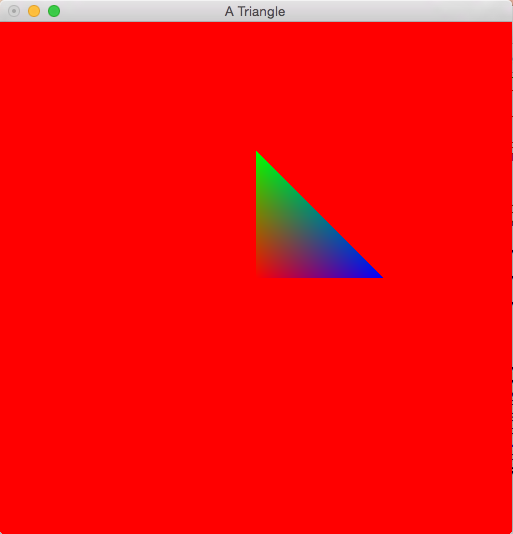
\includegraphics[height=6cm]{OGL_opengl/simpleEx.png}
\end{figure}

\end{frame}

%%%%%%%%%%%%%%%%%%%%%%%%%%%%%%%%%%%%%%%%%%%%%%%%%%%%%%%%%

%%%%%%%%%%%%%%%%%%%%%%%%%%%%%%%%%%%%%%%%%%%%%%%%%%%%%%%%%
\begin{frame}[fragile]{프리미티브(primitives) - 1/3}

\begin{itemize}
\item 그래픽 하드웨어는 프로그래머(programmer)가 지정한 프리미티브(primitive) 설정에 따라 정점의 리스트를 처리
\item 프리미티브는 OpenGL이 제공하는 그리기 기본요소
\item 입력 정점들을 어떻게 조합할 것인가를 결정
\end{itemize}

\begin{itemize}
\item 프리미티브를 사용하는 방법은 다음과 같다.
\end{itemize}

\lstset{language=C++,escapechar=^} 
\begin{lstlisting}
glBegin(^{\sf drawing primitive}^);
      // vertex position, color, normal, etc
      setVertexInfo(); 
glEnd(); 
}

\end{lstlisting}

\end{frame}
%%%%%%%%%%%%%%%%%%%%%%%%%%%%%%%%%%%%%%%%%%%%%%%%%%%%%%%%%

%%%%%%%%%%%%%%%%%%%%%%%%%%%%%%%%%%%%%%%%%%%%%%%%%%%%%%%%%
\begin{frame}[fragile]{프리미티브(primitives) - 2/3}

{\small
\begin{itemize}
\item {\sf GL\_POINTS}: 입력된 정점을 하나씩 점으로 가시화
\item {\sf GL\_LINES}: 입력된 정점을 두 개씩 묶어 선분으로 표현 
\item {\sf GL\_LINE\_STRIP}: 입력된 정점을 차례대로 연결하여 하나의 폴리라인(polyline)을 구성
\item {\sf GL\_LINE\_LOOP}: 입력된 정점을 차례로 연결한 뒤에 마지막 점을 시작점으로 연결
\item {\sf GL\_TRIANGLES}: 입력된 정점을 세 개씩 묶어 삼각형을 그림
\item {\sf GL\_TRIANGLE\_STRIP}: 처음 세 개 정점으로 삼각형을 그린 뒤, 정점이 추가될 때마다 삼각형을 직전 두 개 정점과 연결하여 삼각형 추가 
\item {\sf GL\_TRIANGLE\_FAN}: 부채 모양으로 삼각형을 추가해 나감
\item {\sf GL\_QUADS}: 정점 네 개씩을 묶어 사각형 그리기
\item {\sf GL\_QUAD\_STRIP}: 처음 네 개 정점으로 사각형 그리고, 이후 두 개씩 묵어 직전 두 개 정점과 함께 사각형 그리기
\item {\sf GL\_POLYGON}: 입력된 모든 정점으로 다각형을 그림
\end{itemize}
}


\end{frame}
%%%%%%%%%%%%%%%%%%%%%%%%%%%%%%%%%%%%%%%%%%%%%%%%%%%%%%%%%


%%%%%%%%%%%%%%%%%%%%%%%%%%%%%%%%%%%%%%%%%%%%%%%%%%%%%%%%%
\begin{frame}[fragile]{프리미티브(primitives) - 3/3}

\begin{figure}
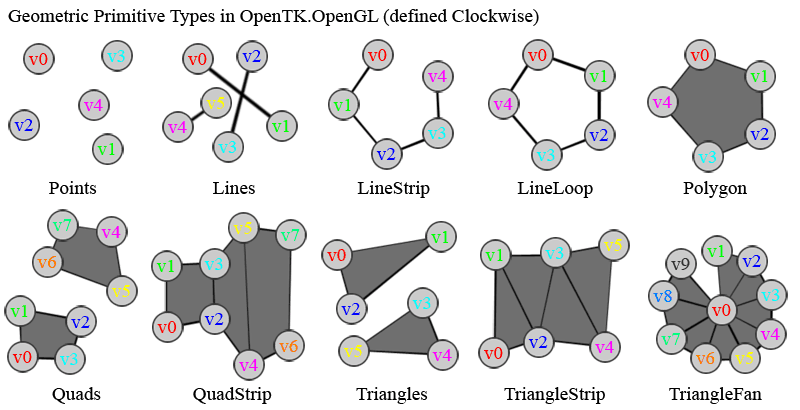
\includegraphics[height=6cm]{OGL_opengl/primitives.png}
\end{figure}


\end{frame}
%%%%%%%%%%%%%%%%%%%%%%%%%%%%%%%%%%%%%%%%%%%%%%%%%%%%%%%%%


%%%%%%%%%%%%%%%%%%%%%%%%%%%%%%%%%%%%%%%%%%%%%%%%%%%%%%%%%
\begin{frame}[fragile]{정점 데이터 설정 방법}

\begin{itemize}
\item 정점 데이터는 위치와 법선벡터, 색 등
\item 정점의 위치만을 입력한다면 glVertex[dim-type]으로 입력
\item 3 차원 정점의 각 성분을 부동소수점 표현으로 넣는다면, glVertex3f(x,y,z)와 같이 입력
\item 다음과 같은 같은 여러 표현이 가능하다.
\end{itemize}

\lstset{language=C++} 
\begin{lstlisting}
float x,y,z;
double dx,dy,dz;
int ix,iy,iz;
float verts = {1.0f, 2.0f, 1.0f};
glBegin(drawing primitive);
      glVertex3f(x,y,z);
      glVertex3d(dx,dy,dz);
      glVertex3i(ix,iy,iz);
      glVertex3fv(verts);
glEnd();
\end{lstlisting}

\end{frame}
%%%%%%%%%%%%%%%%%%%%%%%%%%%%%%%%%%%%%%%%%%%%%%%%%%%%%%%%%

%%%%%%%%%%%%%%%%%%%%%%%%%%%%%%%%%%%%%%%%%%%%%%%%%%%%%%%%%
\begin{frame}[fragile]{다양한 프리미티브를 이용한 풍경 그리기}

    \lstset{language=C++,frame=none,escapechar=^}%
    \foreach \n in {1,26,...,75} {%
       \only<+>{%
            \edef\m{\the\numexpr\n+24\relax}%
            \edef\thesubtitle{{Lines \n--\m\ / 75}}%
            \expandafter\framesubtitle\thesubtitle
            \lstinputlisting[firstline=\n,lastline=\m]{./Codes/L03_sceneWithPrimitives.tex}%
       }%
    }

\end{frame}
%%%%%%%%%%%%%%%%%%%%%%%%%%%%%%%%%%%%%%%%%%%%%%%%%%%%%%%%%

%%%%%%%%%%%%%%%%%%%%%%%%%%%%%%%%%%%%%%%%%%%%%%%%%%%%%%%%%
\begin{frame}[fragile]{다양한 프리미티브를 이용한 풍경 그리기}

\begin{figure}
    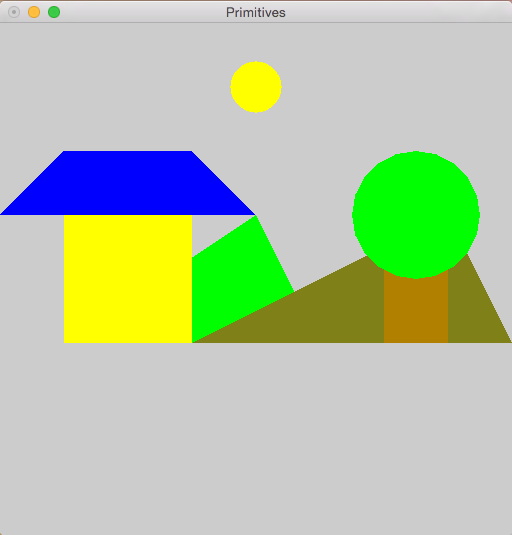
\includegraphics[height=7cm]{OGL_opengl/simpleScene.png}
\end{figure}


\end{frame}
%%%%%%%%%%%%%%%%%%%%%%%%%%%%%%%%%%%%%%%%%%%%%%%%%%%%%%%%%

%%%%%%%%%%%%%%%%%%%%%%%%%%%%%%%%%%%%%%%%%%%%%%%%%%%%%%%%%
\begin{frame}[fragile]{디폴트 카메라}

\begin{itemize}
\item OpenGL의 디폴트 카메라는 원점 위치
\item z축 음의 방향
\item 원근 투영을 적용하지 않아 카메라에 잡히는 공간은 상자 형태
\end{itemize}

\begin{figure}
    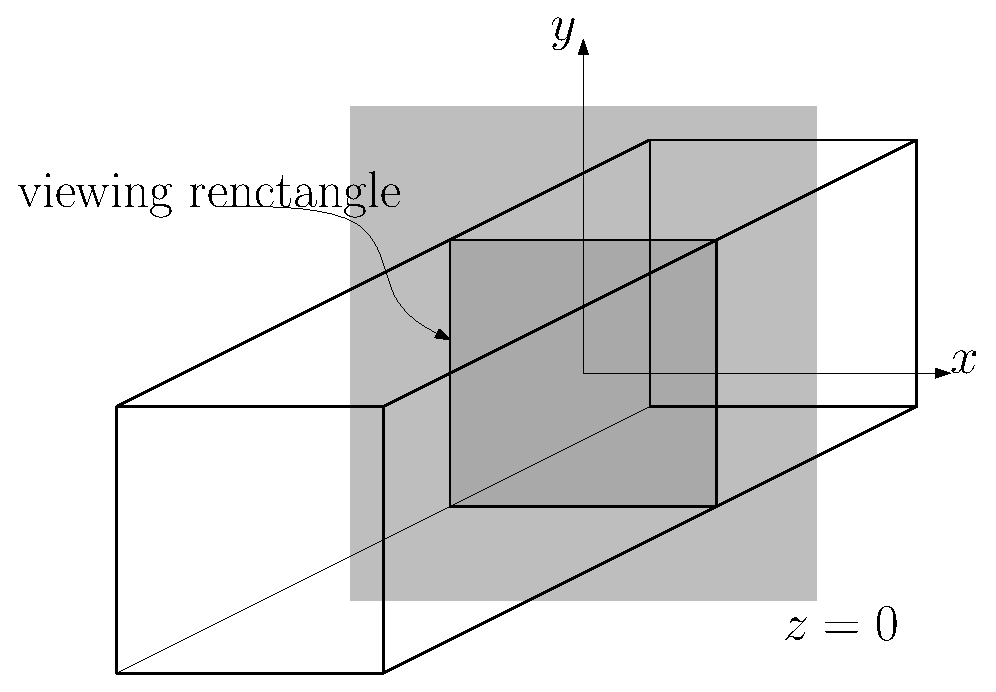
\includegraphics[height=5cm]{OGL_opengl/defaultCam.eps}
\end{figure}


\end{frame}
%%%%%%%%%%%%%%%%%%%%%%%%%%%%%%%%%%%%%%%%%%%%%%%%%%%%%%%%%

%%%%%%%%%%%%%%%%%%%%%%%%%%%%%%%%%%%%%%%%%%%%%%%%%%%%%%%%%
\begin{frame}[fragile]{직교 투영 (orthographics projection) 설정}

\begin{itemize}
\item 디폴트 카메라는 직교 투영 카메라
\item 상자 모양의 가시화 공간내의 객체를 상자를 절단하는 면에 투영
\item 이 상자의 위치와 길이를 변경하는 함수가 glOrtho
\end{itemize}

\begin{figure}
    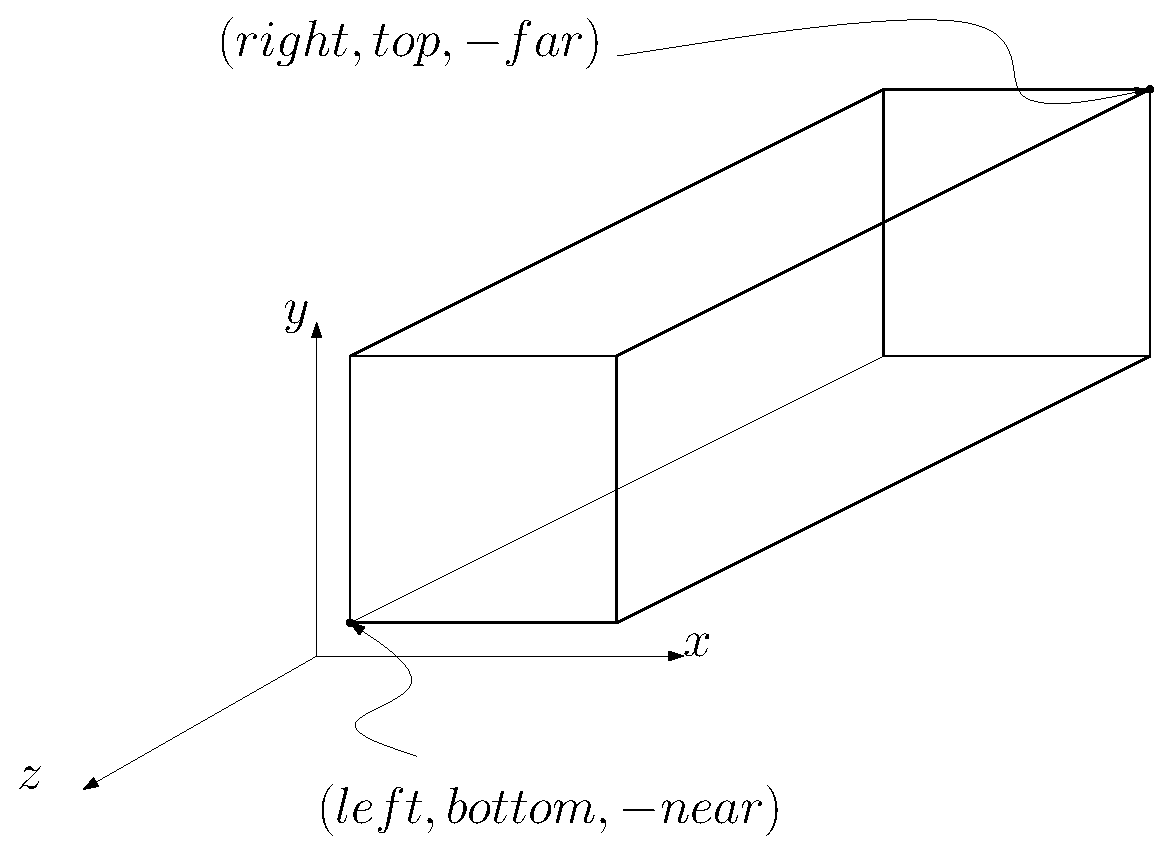
\includegraphics[height=4cm]{OGL_opengl/glOrtho.eps}
\end{figure}
\begin{center}{\tiny glOrtho(float left, float right, float bottom, float top, float near, float far);}
\end{center}

\begin{itemize}
\item 결국 OpenGL의 디폴트 카메라는 다음과 같은 설정
	\begin{itemize}
	\item glOrtho(-1,1, -1,1, -1,1);
	\end{itemize}
\end{itemize}

\end{frame}
%%%%%%%%%%%%%%%%%%%%%%%%%%%%%%%%%%%%%%%%%%%%%%%%%%%%%%%%%

%%%%%%%%%%%%%%%%%%%%%%%%%%%%%%%%%%%%%%%%%%%%%%%%%%%%%%%%%
\begin{frame}[fragile]{원근 투영 (perspective projection) 설정}

{\small
\begin{itemize}
\item 실제 카메라나 우리 눈은 원근이 없는 평행 투영이 불가능
\item 멀리 있는 것은 작게 보이고 가까이 있는 것은 크게 보이는 이유는 원근투영
\item 이러한 원근 투영을 설정하는 방법은 {\sf glFrustum}과 {\sf gluPerspective}
\item {\sf glFrustum}에 대한 이해는 뒤로 미루고 우선 직관적인 {\sf  gluPerspective} 함수를 먼저 이해
\end{itemize}

\begin{verbatim}
gluPerspective(float fovy, float Aspect, float near, float far);
\end{verbatim}


\begin{itemize}
\item {\sf fovy}는 $y$축 방향으로의 시야각을 도(degree)로 나타낸 것
\item {\sf Aspect}는 가시화 볼륨의 종횡비(aspect ratio)
\item {\sf near}는 카메라에서 상이 맺히는 가까운 평면까지의 거리
\item {\sf far}는 가시화 공간을 결정하는 평면 중 카메라에서 가장 먼 쪽 평면과 카메라 사이의 거리
\item 이 함수는 그리기 동작이 일어날 때마다 불리는 것이 아니라 초기에 한 번, 혹은 렌즈를 바꿀 필요가 있을 때에만 불린다.
\end{itemize}
}

\end{frame}
%%%%%%%%%%%%%%%%%%%%%%%%%%%%%%%%%%%%%%%%%%%%%%%%%%%%%%%%%

%%%%%%%%%%%%%%%%%%%%%%%%%%%%%%%%%%%%%%%%%%%%%%%%%%%%%%%%%
\begin{frame}[fragile]{행렬 모드(matrix mode)}

{\small
\begin{itemize}
\item OpenGL은 세 종류의 행렬: 텍스처 행렬, 모델뷰 행렬, 투영행렬
\item 모델뷰 행렬은 공간 내에서 가상 객체의 좌표를 변경
\item 투영행렬은 가상 객체를 투영면에 옮겨 놓음
\end{itemize}

\lstset{language=C++, escapechar=^} 
\begin{lstlisting}
glMatrixMode(GL_PROJECTION);
glLoadIdentity();
gluPerspective(60, 1.0, 0.1, 100.0);

glMatrixMode(GL_MODELVIEW);
glLoadIdentity();
gluLookAt(1.0, 1.0, 1.0, 0.0, 0.0, 0.0, 0.0, 1.0, 0.0);

^{\sf [[draw something]]}^
\end{lstlisting}

\begin{itemize}
\item 여기서는 {\sf gluPerspective}와 {\sf gluLookAt}이 어떠한 행렬 모드을 변경하는가 하는 것이 관심
\item {\sf gluPerspective} 함수는 투영의 특성을 변경하는 것이므로 투영행렬 모드
\item {\sf gluLookAt}은 카메라의 위치를 옮기는 것이고, 이는 바꾸어 말해 물체의 위치를 카메라 기준에서 옮기는 것이므로 모델뷰 행렬을 변경
\end{itemize}
}

\end{frame}
%%%%%%%%%%%%%%%%%%%%%%%%%%%%%%%%%%%%%%%%%%%%%%%%%%%%%%%%%

%%%%%%%%%%%%%%%%%%%%%%%%%%%%%%%%%%%%%%%%%%%%%%%%%%%%%%%%%
\begin{frame}[fragile]{카메라 위치 변경}

\begin{itemize}
\item 카메라를 원하는 곳으로 옮겨주는 함수:  {\sf gluLookAt}
\end{itemize}


\begin{verbatim}
gluLookAt(float eye_x, float eye_y, float eye_z,
          float at_x, float at_y, float at_z,
          float up_x, float up_y, float up_z);
\end{verbatim}


\begin{itemize}
\item 카메라의 위치를 옮겨 놓는 역학
\item 카메라 이동의 반대로 물체를 옮겨 놓는 것
\item 카메라의 위치는 매 프레임마다 변경될 수 있으므로 이 함수는 그리기 함수 내에서 매번 불리는 것이 일반적
\end{itemize}

\end{frame}
%%%%%%%%%%%%%%%%%%%%%%%%%%%%%%%%%%%%%%%%%%%%%%%%%%%%%%%%%

%%%%%%%%%%%%%%%%%%%%%%%%%%%%%%%%%%%%%%%%%%%%%%%%%%%%%%%%%
\begin{frame}[fragile]{카메라를 설정하는 기본적인 프로그램}

    \lstset{language=C++,frame=none,escapechar=^}%
    \foreach \n in {1,26,...,50} {%
       \only<+>{%
            \edef\m{\the\numexpr\n+24\relax}%
            \edef\thesubtitle{{Lines \n--\m\ / 50}}%
            \expandafter\framesubtitle\thesubtitle
            \lstinputlisting[firstline=\n,lastline=\m]{./Codes/L03_simpleCamera.tex}%
       }%
    }

\end{frame}
%%%%%%%%%%%%%%%%%%%%%%%%%%%%%%%%%%%%%%%%%%%%%%%%%%%%%%%%%

\end{document}







\subsection{}



\subsection{카메라의 위치 변경}




\subsection
\begin{algorithmbis}[\label{code:OGL_opengl:SceneWithCam}
\lstset{language=C++, escapechar=^} 
\begin{lstlisting}
^{\sf [[header 파일 포함하기...]]}^

void init(int argc, char **argv) {
  // ^{\it 윈도우 생성, 버퍼 설정}^
  glutInit(&argc, argv);
  glutInitDisplayMode(GLUT_SINGLE|GLUT_RGBA);
  glutInitWindowPosition(0,0);
  glutInitWindowSize(512,512);
  glutCreateWindow("Dr. Kang's Graphics Lecture");
  glClearColor(1.0, 1.0, 1.0, 1.0);
  // ^{\it 카메라 투영 특성 설정 (glPerspective 사용). 이때는 GL\_PROJECTION 행렬모드여야 한다.}^
  glMatrixMode(GL_PROJECTION);
  glLoadIdentity();
  gluPerspective(60, 1.0, 0.1, 100.0);
}

void drawScene() {
  ^{\sf [[앞서 사용한 코드 \ref{code:OGL_opengl:simpleScene}의 그리기 코드를 여기에 넣는다. (단, glFlush는 여기서 사용하지 않는다)]]}^
}
void drawAxes() {
  glBegin(GL_LINES);
  glColor3f(1.0, 0.0, 0.0);
  glVertex3f(0.0, 0.0, 0.0);   glVertex3f(1.0, 0.0, 0.0);
  glColor3f(0.0, 1.0, 0.0);
  glVertex3f(0.0, 0.0, 0.0);  glVertex3f(0.0, 1.0, 0.0);
  glColor3f(0.0, 0.0, 1.0);
  glVertex3f(0.0, 0.0, 0.0);  glVertex3f(0.0, 0.0, 1.0);
  glEnd();
}

void display() {
  static float t=0.0;
  // ^{\it 카메라의 위치와 방향을 설정한다. 이때는 GL\_MODELVIEW 행렬 모드여야 한다.}^
  glMatrixMode(GL_MODELVIEW);
  glLoadIdentity();
  gluLookAt( 2.0*sin(t), 1, 2.0*cos(t), 0, 0, 0,  0, 1, 0);
  t+=0.001;
  glClear(GL_COLOR_BUFFER_BIT);
  drawScene();		
  glLineWidth(5);
  drawAxes();		
  glLineWidth(1);
  glFlush();
};

int main (int argc, char **argv) {
  init(argc, argv);
  glutDisplayFunc(display);
  glutIdleFunc(display);
  glutMainLoop();
}
\end{lstlisting}
\end{algorithmbis}

코드. \ref{code:OGL_opengl:SceneWithCam}를 통해 얻을 수 있는 결과는 그림. \ref{fig:OGL_opengl:camMove}를 통해 확인할 수 있다.
이 코드를 실행하면 앞서 그렸던 평면적인 장면이 3차원 공간에서 입체적으로 회전하는 모습을 볼 수 있다.
코드의 의미를 해석하자면, $xz$ 평면에서 원점을 중심으로 반지름 2.0인 원의 원주 위에 카메라를 두고 원주를 따라 돌면서
쳐다보는 방향은 원점으로 고정한 것이다. 공간을 좀 더 잘 확인할 수 있도록 세 개의 축을 그려 넣었다.

\begin{figure}[h!]
  \centering
    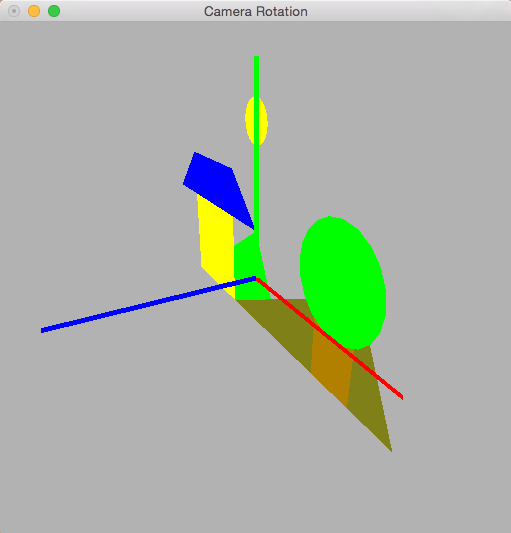
\includegraphics[height=10cm]{OGL_opengl/camMove.png}
    \caption{카메라의 위치와 방향이 변경된 결과}
    \label{fig:OGL_opengl:camMove}
\end{figure}

\section{입체와 깊이 버퍼의 활용}

앞 절에서 카메라를 옮겨 보았다. 이를 통해 우리가 그리고 보는 공간이 3차원 공간임을 확인할 수 있었다. 그러나, 아직은 납작한 평면에 그림을 그리고 돌려본 상태이다. 부피를 가진 입체 도형을 그리는 것이 이 절의 주제이다.
좌표를 3차원으로 설정하면 입체는 그려진다. 2차원 그리기와 전혀 다를 바가 없는 문제이다. 그러나 여기에서 우리는 새로운 문제를 만나게 된다.
다음의 크드. \ref{code:OGL_opengl:3DObjects}와 같은 그리기 코드가 있다. {\sf display} 함수에서 
이 코드에 나타나 있는 {\sf draw} 함수를 호출하면 어떤 그림이 그려질지 상상해 보자.


이 그리기 코드는 노란색 뚜껑과, 하늘색 바닥이 있고, 왼쪽에는 초록색 벽, 오른쪽에는 흰색 벽을 그리고, 입체 안에 3 개의 축을 그리는 코드이다. 그런데 앞서 작성된 코드의 {\sf display} 콜백 함수 내에 {\sf draw()}를 삽입하면 그림. \ref{fig:OGL_opengl:noZBuff}와 같이 그려진다.
지정한 좌표에 제대로 그려진 것 같지만 자세히 살펴보면 무엇인가 이상하다.

\begin{algorithmbis}[입체 도형 그리기 예제]\label{code:OGL_opengl:3DObjects}
\lstset{language=C++, escapechar=^} 
\begin{lstlisting}
void drawScene() {
  // drawing code
  glBegin(GL_QUADS);
  // ^{\it 천정}^
  glColor3f(1.0, 1.0, 0.0);
  glVertex3f(-0.5, 0.5, -0.5);
  glVertex3f( 0.5, 0.5, -0.5);
  glVertex3f( 0.5, 0.5,  0.5);
  glVertex3f(-0.5, 0.5,  0.5);
  // ^{\it 바닥}^
  glColor3f(0.0,1.0,1.0);
  glVertex3f(-0.5,-0.5, -0.5);
  glVertex3f( 0.5,-0.5, -0.5);
  glVertex3f( 0.5,-0.5,  0.5);
  glVertex3f(-0.5,-0.5,  0.5);
  // ^{\it 왼쪽 벽}^
  glColor3f(0.0,1.0,0.0);
  glVertex3f(-0.5, 0.5, -0.5);
  glVertex3f(-0.5, 0.5,  0.5);
  glVertex3f(-0.5,-0.5,  0.5);
  glVertex3f(-0.5,-0.5, -0.5);
  // ^{\it 오른쪽 벽}^
  glColor3f(1.0,1.0,1.0);
  glVertex3f( 0.5, 0.5, -0.5);
  glVertex3f( 0.5, 0.5,  0.5);
  glVertex3f( 0.5,-0.5,  0.5);
  glVertex3f( 0.5,-0.5, -0.5);
  glEnd();
}

void draw() {
  drawScene();
  drawAxes(); //^{\it drawAxes 함수는 코드 \ref{code:OGL_opengl:SceneWithCam}에서 사용한 것을 그대로 쓴다.}^
}
\end{lstlisting}
\end{algorithmbis}


\begin{figure}[h!]
  \centering
    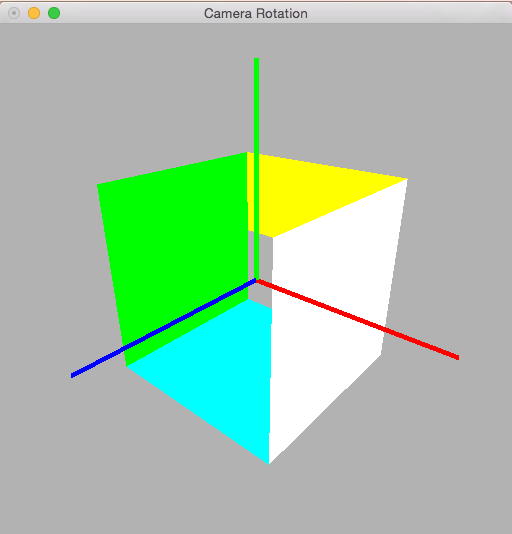
\includegraphics[height=10cm]{OGL_opengl/noZBuff.png}
    \caption{입체의 깊이가 고려되지 않은 결과}
    \label{fig:OGL_opengl:noZBuff}
\end{figure}

노란색 뚜겅이 뒤에 있는 초록색 벽에 가려지는 현상이 발생하며, 벽이나 뚜껑에 의해 일부가 가려져야 하는 축이 전혀 가려지지 않고 그려지고 있다.
이 문제는 OpenGL에게 그려지는 픽셀의 깊이를 고려하도록 하지 않을 경우에 발생하는 문제이다.
OpenGL에게 그려진 픽셀의 깊이를 고려하라고 하지 않았기 때문에 지금 그리려고 하는 객체의 픽셀이 
이미 그려진 객체에 가려지는지를 검사하지 않는 것이다.
이럴 경우 가장 나중에 그려진 것은 다른 객체와의 깊이를 따지지 않고 무조건 화면에 나타나게 된다.
예를 들어 이 코드에서는 축이 가장 나중에 그려졌기 때문에 어느 누구에게도 가려지지 않는다.
이러한 문제는 깊이 버퍼를 사용하여 해결할 수 있다.

\subsection{깊이 버퍼(depth buffer)의 사용}

\index{z-buffer}\index{color buffer}
\index{z-버퍼}\index{색상 버퍼}
z-버퍼라고도 불리는 깊이 버퍼는 영상을 생성할 때에 사용되는 여러 버퍼 가운데 하나이다. 가장 일반적인 버퍼는 색상 버퍼(color buffer)인데, 그려지는 영상의 각 화소별 색을 기록하는 것이다. 우리가 최종적으로 보게되는 것은 이 색상 버퍼의 내용이 된다. 그런데, 이런 색상 버퍼를 구성할 때 물체의 가려짐을 고려하여 가려진 물체를 그리지 않도록 해야 하는데, 이를 해결하는 버퍼가 깊이 버퍼이다. 깊이 버퍼는 객체를 그릴 때, 색상이 아니라 카메라에서 그려지는 픽셀까지의 거리를 저장하는 버퍼이다. 그림. \ref{fig:OGL_opengl:Z_Buffer}는 그래픽스 프로그램에서 일반적으로 가시화되는 색상 버퍼의 내용과, 이 장면에 해당하는 깊이 버퍼를 비교하고 있다.

\begin{figure}[h!]
  \centering
    \includegraphics[height=10cm]{OGL_opengl/Z_Buffer.png}
    \caption{가시화되는 색샹 버퍼의 내용과 객체의 깊이 정보를 담은 z-버퍼의 비교}
    \label{fig:OGL_opengl:Z_Buffer}
\end{figure}


깊이 버퍼가 있다면 어떤 픽셀을 그릴 때에 이미 그려진 픽셀의 깊이를 보고 이 깊이 값보다 새로 그리려는 픽셀의 깊이값이 카메라에서 가까운 값일 경우에만 그림을 그린다. 이 방법은 일반적으로 하드웨어를 통해 이루어진다.
깊이 버퍼를 사용함으로써 우리는 효율적으로 가려져서 보이지 않는 물체를 렌더링에서 제외시킬 수 있다. 
OpenGL에서는 이러한 깊이 버퍼를 쉽게 사용할 수 있도록 지원한다. GLUT 라이브러리를 사용한다고 가정하면 {\sf glutInitDisplayMode} 함수를 이용하여 다음과 같이 설정하면 깊이 버퍼를 사용할 수 있다.

\begin{itemize}
\item{\sf glutInitDisplayMode(GLUT\_SINGLE $|$ \color{red}{GLUT\_DEPTH} $|$ GLUT\_RGBA);}
\end{itemize}

\index{GL\_DEPTH\_TEST}
하지만 이렇게 깊이 버퍼를 사용한다고 해서 깊이 버퍼를 활용하여 가려진 물체를 렌더링에서 제외하는 작업이 이루어지지는 않는다. OpenGL은 기본적으로 깊이를 검사하는 “깊이 테스트” 작업을 수행하지 않는 것이 디폴트 상태이기 때문이다. 깊이 테스트를 수행하기 위해서는 다음과 같이 상태를 변경해야 한다.

\begin{itemize}
\item{\sf glEnable(\color{red}{GL\_DEPTH\_TEST});}
\end{itemize}

또한 매번 그리기가 이뤄지면 그려진 내용에 따라 깊이 버퍼의 내용이 더러워져 있는 상태가 되므로, 새로운 그리기를 하기 전에 색상 버퍼를 깨끗하게 지우듯이 깊이 버퍼의 내용도 깨끗하게 지우는 다음과 같은 코드가 필요하다.

\index{GL\_DEPTH\_BUFFER\_BIT}
\begin{itemize}
\item{\sf glClear( GL\_COLOR\_BUFFER\_BIT $|$ \color{red}{GL\_DEPTH\_BUFFER\_BIT});}
\end{itemize}
이상과 같이 깊이 버퍼의 설정과 깊이 테스트를 수행하도록 상태를 변경하면 앞서의 결과는 다음과 같이 기대했던 것과 같이 그려지게 된다.
그림에서 축은 자연스럽게 뚜겅과 우측 벽에 의해 가려지고 있으며, 좌측 벽도 뚜껑에 가려져 나타나게 된다.


\subsection{이중 버퍼의 사용}

\index{이중 버퍼}\index{double buffering}
우리는 지금까지 색상과 깊이 버퍼가 하나만 존재하는 단일 버퍼 환경에서 작업을 하였다. 그런데 이러한 단일 버퍼 환경은 애니메이션 등이 있을 때 하나의 버퍼를 다 지우고 새로운 그림을 그리는 과정에서 화면 깜빡임이 있을 수 있다.
화면 깜빡임을 해결하는 방법은 버퍼를 앞 버퍼(front buffer)와 뒷 버퍼(back buffer)의 이중 구조로 만들어 앞 버퍼가 출력되고 있을 때 다음에 보여질 그림은 뒷 버퍼에 그리는 것이다. 그리고 뒷 버퍼의 그림이 다 그려지고 화면에 보여질 준비가 마쳤을 때, 앞 버퍼와 뒷 버퍼의 역할을 뒤바꾸는 버퍼 스와핑(swaping)을 수행하는 것이다. 지금부터 본 자료의 모든 코드는 이러한 이중 버퍼의 사용을 기본으로 하겠다. 

\index{GL\_SINGLE}\index{GL\_DOUBLE}
이중 버퍼를 실제로 사용하는 방법은 다음과 같이 우선 glutInitDisplayMode 함수에서 {\sf GL\_SINGLE}을 {\sf GL\_DOUBLE}로 바꾸어 시스템이 두 개의 버퍼를 준비하게 하는 것이다.

\begin{itemize}
\item {\sf glutInitDisplayMode( \color{red}{GLUT\_DOUBLE} $|$ GLUT\_DEPTH $|$ GLUT\_RGBA);}
\end{itemize}

\index{glutSwapBuffers}
또한 버퍼의 송출은 {\sf glFlush}가 아니라 {\sf glutSwapBuffers}를 이용한다.

\begin{itemize}
\item {\sf glutSwapBuffers();}
\end{itemize}

이상과 같은 방법을 통해 화면의 깜박임이 업는 이중 버퍼링 활용이 가능하다. 지금까지의 내용을 정리하여 소스코드는 다음 코드. \ref{code:OGL_opengl:3DObjectsWithZbuff}와 같이 애니메이션 되는 이중버퍼-깊이버퍼 사용 예제 코드로 개선이 가능하다.

이때 {\sf keyboard}라는 함수가 추가로 구현되었고, 이를 {\sf glutKeyboardFunc}를 이용하여 키보드 처리 콜백 함수로 사용하고 있다. 이 내용은 쉽게 이해할 수 있으므로 설명을 생략한다. 다만 이 함수 안에 있는 {\sf glutPostRedisplay} 함수에 대한 설명이 필요한데, 이 함수는 사용자가 강제로 그리기 이벤트를 발생 시키는 것이다. 즉 키보드 입력이 있으면 자동으로 그려지기가 불리게 된다.

\begin{algorithmbis}[애니메이션이 포함된 깊이버퍼/이중버퍼 활용 예제]\label{code:OGL_opengl:3DObjectsWithZbuff}
\lstset{language=C++, escapechar=^} 
\begin{lstlisting}

^{\sf [[헤더 파일 포함하기]]}^

void init(int argc, char **argv) {
    // ^{\it 윈도우 생성, 버퍼 설정}^
    glutInit(&argc, argv);
    // ^{\it 이중 버퍼링, RGBA 색상 버퍼와 함께, 깊이 버퍼를 준비하도록 한다.}^
    glutInitDisplayMode(GLUT_DOUBLE|GLUT_RGBA|GLUT_DEPTH);
    glutInitWindowPosition(0,0);
    glutInitWindowSize(512,512);
    glutCreateWindow("DEPTH BUFFER");
    glClearColor(0.7, 0.7, 0.7, 1.0);
    // ^{\it 깊이 버퍼 검사를 활성화한다.}^
    glEnable(GL_DEPTH_TEST);
    // ^{\it 카메라 투영 특성 설정 (glPerspective 사용). 이때는 GL\_PROJECTION 행렬모드여야 한다.}^
    glMatrixMode(GL_PROJECTION);
    glLoadIdentity();
    gluPerspective(60, 1.0, 0.1, 100.0);
}
void drawScene() {     ^{\sf [[코드 \ref{code:OGL_opengl:3DObjects}와 동일]]}^  }
void drawAxes() {     ^{\sf [[코드 \ref{code:OGL_opengl:3DObjects}와 동일]]}^ }
void draw() { ^{\sf [[코드 \ref{code:OGL_opengl:3DObjects}와 동일]]}^  }
void display() {
    static float t=0.0;
    // ^{\it 카메라의 위치와 방향을 설정한다. 이때는 GL\_MODELVIEW 행렬 모드여야 한다.}^
    glMatrixMode(GL_MODELVIEW);
    glLoadIdentity();
    gluLookAt( 2.0*sin(t), 1, 2.0*cos(t), 0, 0, 0,  0, 1, 0);
    t+=0.001;
    // ^{\it 컬러 버퍼 뿐만 아니라 깊이 버퍼도 매 프레임마다 지운다.}^
    glClear(GL_COLOR_BUFFER_BIT|GL_DEPTH_BUFFER_BIT);
    draw();
    glutSwapBuffers();
};
\end{lstlisting}
\end{algorithmbis}

이상의 코드를 수행하면, 그림. \ref{fig:OGL_opengl:ZBuff}와 같이 3차원 공간에서 각각의 객체가 시점으로부터 얼마나 떨어져 있는지를 비교하여 뒤에 있는 물체가 앞의 물체에 의해 가려지는 효과를 잘 표현할 수 있다.

\begin{figure}[h!]
  \centering
    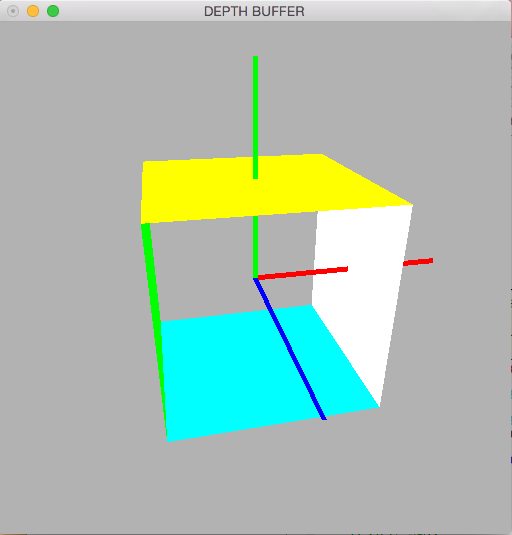
\includegraphics[height=10cm]{OGL_opengl/ZBuff.png}
    \caption{z-버퍼를 이용한 객체의 깊이 비교 적용 결과}
    \label{fig:OGL_opengl:ZBuff}
\end{figure}
 
OpenGL에 대한 소개는 \cite{woo1999openGL,wright2004openGL} 등을 참고하라.


